\documentclass{article} % For LaTeX2e
\usepackage{nips15submit_e}
\usepackage{hyperref}
\usepackage{url}
\usepackage{float}
\usepackage{graphicx}
\usepackage{caption}
\usepackage{subcaption}
\usepackage{capt-of}
\usepackage{amsfonts}

%\font\tinyclef=musix20 scaled 500
%\documentstyle[nips14submit_09,times,art10]{article} % For LaTeX 2.09


\title{Making Music with Hidden Markov Models}


\author{
Anna Yanchenko \\
Duke University\\
\texttt{anna.yanchenko@duke.edu} \\
\And
Megan Robertson \\
Duke University \\
\texttt{megan.robertson@duke.edu} \\
}

\hypersetup{
    colorlinks=true,
    linkcolor=blue,
    filecolor=magenta,      
    urlcolor=cyan,
    pdftitle={Sharelatex Example},
    bookmarks=true,
    pdfpagemode=FullScreen,
}

\newcommand{\fix}{\marginpar{FIX}}
\newcommand{\new}{\marginpar{NEW}}

\nipsfinalcopy % Uncomment for camera-ready version



\begin{document}


\maketitle

\begin{abstract}
Hidden Markov Models (HMMs) are widely used  for modeling sequential data and have many varying applications.  In this project, we use HMMs to capture the latent elements involved in music creation. The observed states are the pitch and velocity (volume) of each note in an existing  song, while the latent states include elements such as chord progression, harmonics, dynamics and melody.  In this paper, we implement three different Hidden Markov Models trained on classical piano pieces and compare the resulting compositions for each model. 
\end{abstract}
 
\section{Introduction}

Hidden Markov Models are known for their use in language applications such as speech recognition and handwriting recognition programs. Inspired by a recent homework assignment using Hidden Markov Models to generate text, we wanted to explore how successful these same models would be in generating music. Thus, this project served as a platform to combine our shared interests of music and statistics. 

This project used music data in the form of MIDI (Musical Instrument Digital Interface) files. This interface creates a form of communication between computers and musical instruments that enables them to send instructions back and forth. MIDI files can contain multiple channels that store information about the notes and velocities of different instruments.   Each note's pitch is coded as an integer between 0 and 127, where 60 refers to middle C.  The velocities are also coded as integers from 0 to 127. The files additionally contain information about when a particular note starts and stops.\footnote{MIDI Manufacturers Association, "An Introduction to MIDI"} 


Much thought and musical theory goes into composing any piece.  The notes must progress in a logical, harmonic way that is pleasing to the listener. The composer must pay close attention to the circle of fifths to determine which notes sound musically cohesive.  Dissonance can be used to elicit specific moods in the piece but does not occur by chance.  In addition, the composer must use melody, harmonies and dynamics to create a piece of music that tells a story or conjures a specific emotion in the listener.\footnote{Music Composition for Dummies, \url{http://www.dummies.com/how-to/content/music-composition-for-dummies-cheat-sheet.html}}

However, the MIDI data of a note's pitch and velocity in sequential order alone does not capture all of the theory and ideas that create a composition. Therefore, we used Hidden Markov Models (HMMs) to model the latent variables, specifically the musical theory that goes into composing a piece. We utilized three different HMMs and trained them on classical piano pieces. The estimated parameters were then used to generate new music based on the modeling of the original piece.  Our goal was to compare how successful each of the three HMMs was in generating a musically pleasing piece and how similar our generated music was to the original composition.

\section{Methods}

Classical piano pieces were used to train each of the models. In this paper we present the results for Gustav Holst's Jupiter from "The Planets" (arranged for piano) and Johann Pachelbel's Canon in D. The MIDI files for these songs were converted to Comma Separated Value (CSV) files.\footnote{This was done using a program found at \url{http://www.fourmilab.ch/webtools/midicsv/}} 

The classical pieces were used to estimate the respective parameters of the models described below. In this training, the tempo, key signature and length of the original song were not changed. The only possible observed states were the velocities and note pitches present in the original pieces. We treated the pitch of each note and its velocity as independent variables.  Once the parameters had been estimated, they were used to generate a new piece of music. This process generated a CSV file of the new composition and this file was then converted back to a MIDI file using the same program as above. The files could then be played using a synthesizer or a program such as GarageBand.

The three models that we considered were a first order HMM, a second order HMM and a first order HMM with two hidden states.  We used the Baum-Welch algorithm  to estimate the parameters in our model, where $\{X_t\}$ were the observed states and $\{Z_t\}$ were the hidden states, $t = 1, \cdots, T$.  The three models used the following parameters: the initial distribution, $\pi_i = \mathbb{P}(Z_1 = i)$, the transition matrix, $T_{ij} = \mathbb{P}(Z_{t+1} = j | Z_t = i)$ and the emission distribution, $\phi_i (X_t) = p(X_t | Z_t = i)$. For each of the three models, we assumed that each $Z_t$ could take $m$ possible discrete states and that each $X_t$ could take $k$  possible discrete states, where $1, \cdots, k$ corresponded to the note pitches or velocities occurring in the original piece. For example, if the original piece had 10 different note pitches and 5 different velocities, $k=10$ for the HMM run on the observed notes (with each state corresponding to a specific one of those 10 unique pitches) and $k=5$ for the HMM run on the observed velocities.  
The model was run once for note velocities and once for note pitches, independently. 

The Baum-Welch algorithm was adjusted from the  first order form to take into account the structure of the parameters in the second order and two hidden state models.   Using the parameters estimated from the Baum-Welch algorithm, a new song was generated for each of the three models. In order to evaluate the performance of each model, twenty-two survey respondents determined which of the compositions generated using the three different HMMs they liked best, for either Pachelbel's Canon or Holst's Jupiter. They were also provided  the original versions for both Jupiter and Pachelbel's Canon and were asked which of the original versions they thought inspired the remixes. 

\subsection {Model 1: First Order Hidden Markov Model}

The simplest of the three models was the first order Hidden Markov Model. In this model, the observed values, $X_t$, were the notes' pitch or their velocity (modeled independently). The model had only one hidden state, $Z_t$, for each pitch or velocity  and each hidden state only depended on the prior hidden state (\autoref{oneGM}). This model was run using $m = 75$ hidden states.

\begin{figure}[H]
\begin{center}


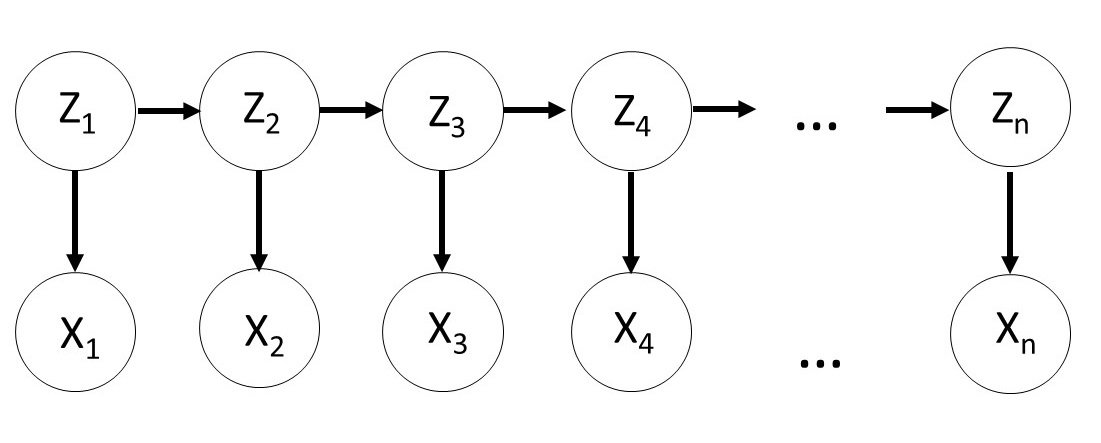
\includegraphics [scale = 0.35] {Model1.jpg}

\caption{Graphical Model - First Order HMM \label{oneGM}}
\end{center}
\end{figure}

The Baum-Welch Algorithm as derived in class was used to estimate the parameters of this model. For details of the derivations and algorithm of this first order HMM see the class notes.\footnote{Statistics 531, Duke University Spring 2016. Instructor: Jeff Miller}
 
\subsection{Model 2: Second Order Hidden Markov Model}

The second order HMM assumed that each hidden state  depended on the two previous  states (\autoref{2HMM}). This enabled the model to capture more of the musical structure inherent in the piece, since this structure was evolving over time and depended on more than just the previous note. The Baum-Welch Algorithm was again used to estimate the parameters, this time modified to accommodate the addition of another transition matrix, $$T_{ijk} = \mathbb{P}[Z_t = k | Z_{t-1} = j, Z_{t-2} = i]$$ which modeled the dependence of the current hidden state on the two previous hidden states. The details of the algorithm for this model can be found in Mari and Schott's "Probabilistic and Statistical Methods in Computer Science"\footnote{Jean-Francoix Mari and Rene Schott, "Probabilistic and Statistical Methods in Computer Science", Springer Science, pg. 161-167 and Brett Watson and Ah Chung Tsoi, "Second Order Hidden Markov Models for Speech Recognition", University of Queensland.}, with a summary of the main results in the Appendix (\autoref{2ndHMM}). This model was run with $m = 50$ hidden states. Fewer states were used than with Model 1 due to computational limitations.

\begin{figure}[H]
\centering

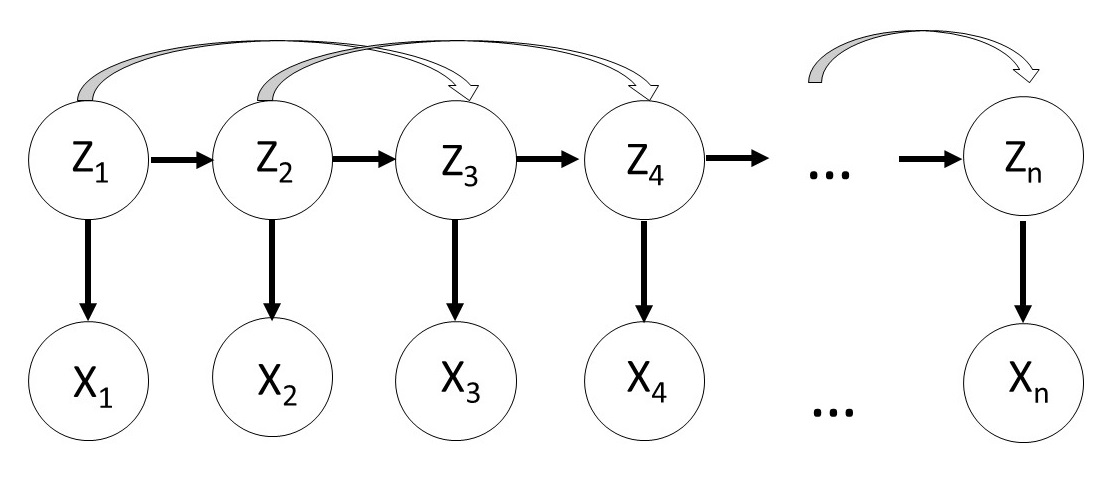
\includegraphics [scale = 0.35] {Model2.jpg}
\caption{Graphical Model - Second Order HMM\label{2HMM}}
\end{figure}

\subsection{Model 3: HMM with Two Hidden States}

The final model expanded on the initial model by adding a second hidden state (\autoref{3HMM}). This meta-state allowed the model to capture additional aspects of the hidden states and the music generation process.  These processes might have evolved at a rate different than the processes that were present in the observed states and the first latent state.  This HMM involved a specific form of the transition matrix that allowed for a more efficient implementation of the derived Baum-Welch algorithm.  In particular, we assumed that the transition matrix factored as
$$T_{ik, jl} = A_{ij}B_{jkl} = \mathbb{P}(R_t = j, S_t = l | R_{t-1} = i, S_{t-1} = k),$$
where $A_{ij} = \mathbb{P}(R_t = j | R_{t-1} = i)$ and $B_{jkl} = \mathbb{P}(S_t = l | R_t = j, S_{t-1} = k)$.  A full derivation for the Baum-Welch algorithm for this model can also be found in the Appendix (\autoref{3rdHMM}). For each hidden state $S_t$, there were ten possible hidden states and for each hidden state $R_t$, there were fifteen possible hidden states . These numbers were kept small so that the parameters could be computed in a reasonable amount of time.

\begin{figure}[H]
\centering

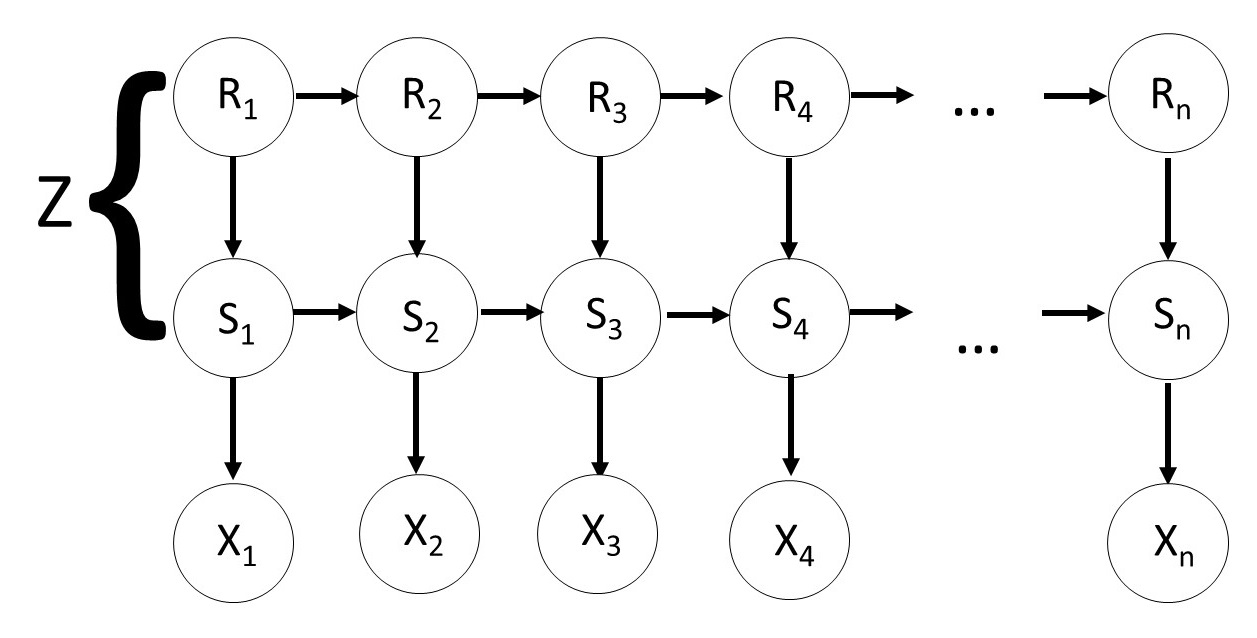
\includegraphics [scale = 0.35] {Model3.jpg}
\caption{Graphical Model - First Order HMM with Two Hidden States\label{3HMM}}
\end{figure}


\section{Results}

\subsection{Original Pieces}

The three models were originally trained on four different classical piano pieces (or orchestral pieces arranged for piano).  These four pieces included Claude Debussy's Clair de Lune and Antonin Dvorak's Largo from Symphony No. 9 ("The New World"), in addition to Jupiter and Pachelbel's Canon.  Of the four pieces, Jupiter and Pachelbel's Canon provided the best results for all of the HMMs considered. It is possible that these pieces performed the best because of their prominent melody from the beginning of the file used. For example, in  Clair de Lune, the piece builds for a while before the melody emerges, while the version of Jupiter that we used to train the models featured just the main melody. Thus the melody did not have to build over a long period of time. Our models may not have worked well for these longer songs because the models did not have the capability to capture the building structure and evolving melody of the song over a long stretch of notes.  

Both Jupiter and Pachelbel's Canon are well-known classical pieces whose themes occur frequently in advertisements and other media forms. The two pieces have a logical musical progression. It is obvious that these pieces are structurally sound and musically cohesive given their popularity. 

 A sample of the sheet music for the first 13 measures of Jupiter in it's original form is included below (\autoref{Jorig}).  The top row of each line is usually played by the right hand of the piano player and is written in Treble Clef (\autoref{keys}), while the bottom row of each line is usually played by the left hand and is written in Bass Clef  (lower than Treble Clef)\footnote{\url{http://www.guitarsite.de/p1042.htm}}. The two lines are played at the same time, thus there are 13 measures included in this original sheet music.  A sample of the sheet music for Pachelbel's Canon is included in the Appendix (\autoref{Jorig}).
 

 
 
 \begin{figure}[H]
\centering

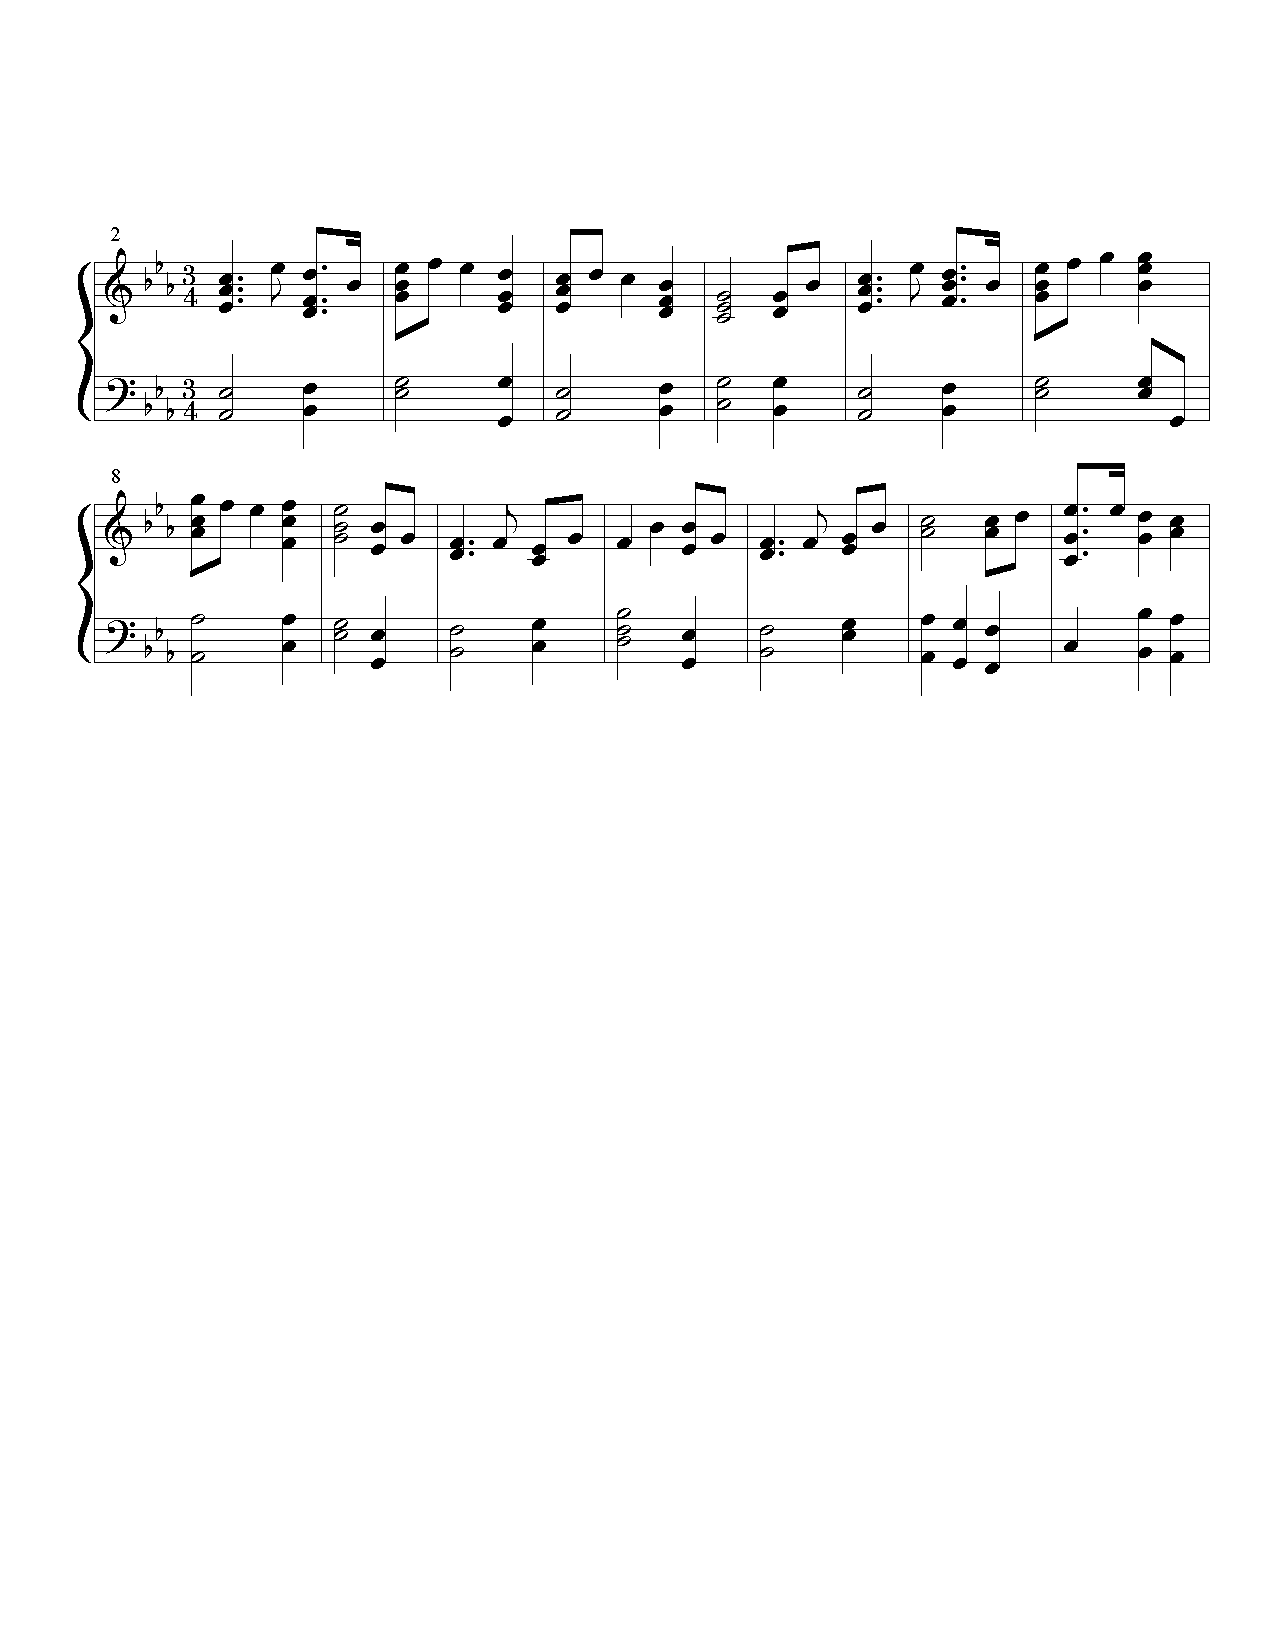
\includegraphics [scale = 0.6] {JupiterOriginal-cropped.pdf}
\caption{Jupiter - Original Song\label{Jorig}}
\end{figure}

\begin{figure}[H]
\centering

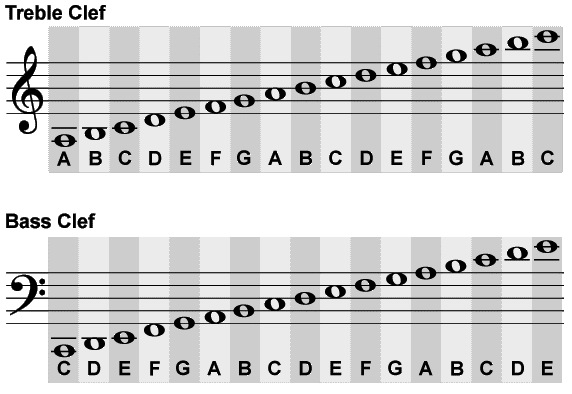
\includegraphics [scale = 0.6] {clef.jpg}
\caption{Musical Clefs: Treble Clef and Bass Clef\label{keys}}
\end{figure}


\subsection{Model 1: First Order Hidden Markov Model}

The Jupiter remix created using the first order Hidden Markov Model had lots of octave and large pitch interval jumps that were not present in the original song. For example, in measures one, three and four in the sheet music for the piece generated by this model (\autoref{J1}),  pitches jump over an octave or more from one note to the next.  In addition, there were more rests in the first two lines of the remix and there were also more quarter and half notes than occurred in the original piece. The melody of the song seemed to be distributed about equally between the left and the right hands, while in the original composition the right hand had the entire melody, while the left hand played the accompaniment.  There was also no musical resolution at the end of this remix.

\begin{figure}[H]
\centering

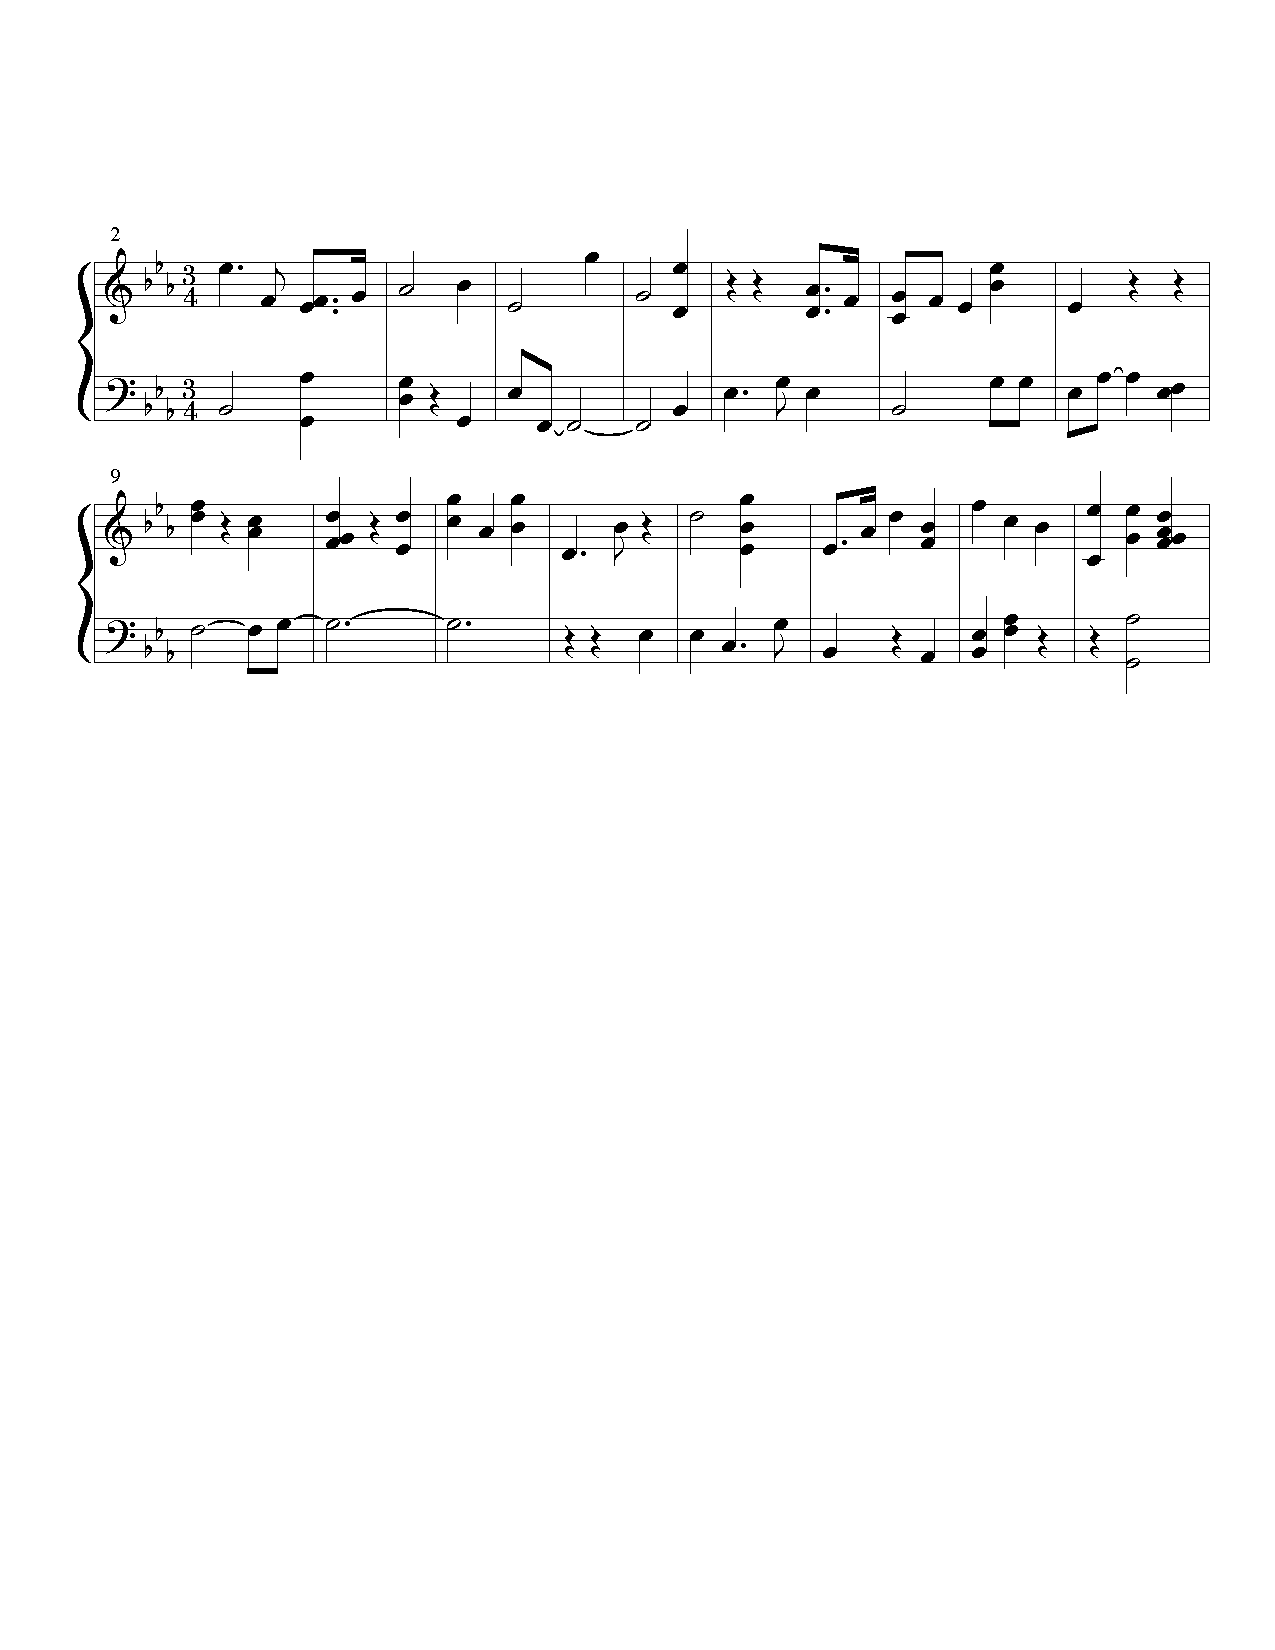
\includegraphics [scale = 0.6] {JupiterRemix-cropped.pdf}
\caption{Jupiter Remix - Model 1\label{J1}}
\end{figure}

The remixed version of Pachelbel's Canon had less sixteenth notes but more dotted notes than the original piece. Pachelbel's Canon consists of mostly eighth or sixteenth notes for the melody. There were also more rests in this remixed version than there are in the original. Finally, there were  octave jumps and jumps of large pitch intervals in this version (\autoref{P1}).

The first order HMM compositions sounded very different from the original compositions. This probably occurred because the model did not capture enough of the overall structure of the original piece. Thus there  were some notes that occurred together that musically should not have, leading to dissonance, while  there is no dissonance in the original songs. For example, the melody for Pachelbel's Canon builds over several measures, yet our first order HMM was not able to capture enough of this building structure to generate an analogous progressing melody. 


\subsection{Model 2: Second Order Hidden Markov Model}

The Jupiter composition created using the second order Hidden Markov Model was an improvement on the first remix. It still had some large interval jumps in terms of pitch, but fewer jumps than Model 1 (\autoref{J2}). The chords also made more sense in the piece and there was less dissonance. The piece also had fewer rests than the first order composition, but more rests than in the original composition.


\begin{figure}[H]
\centering

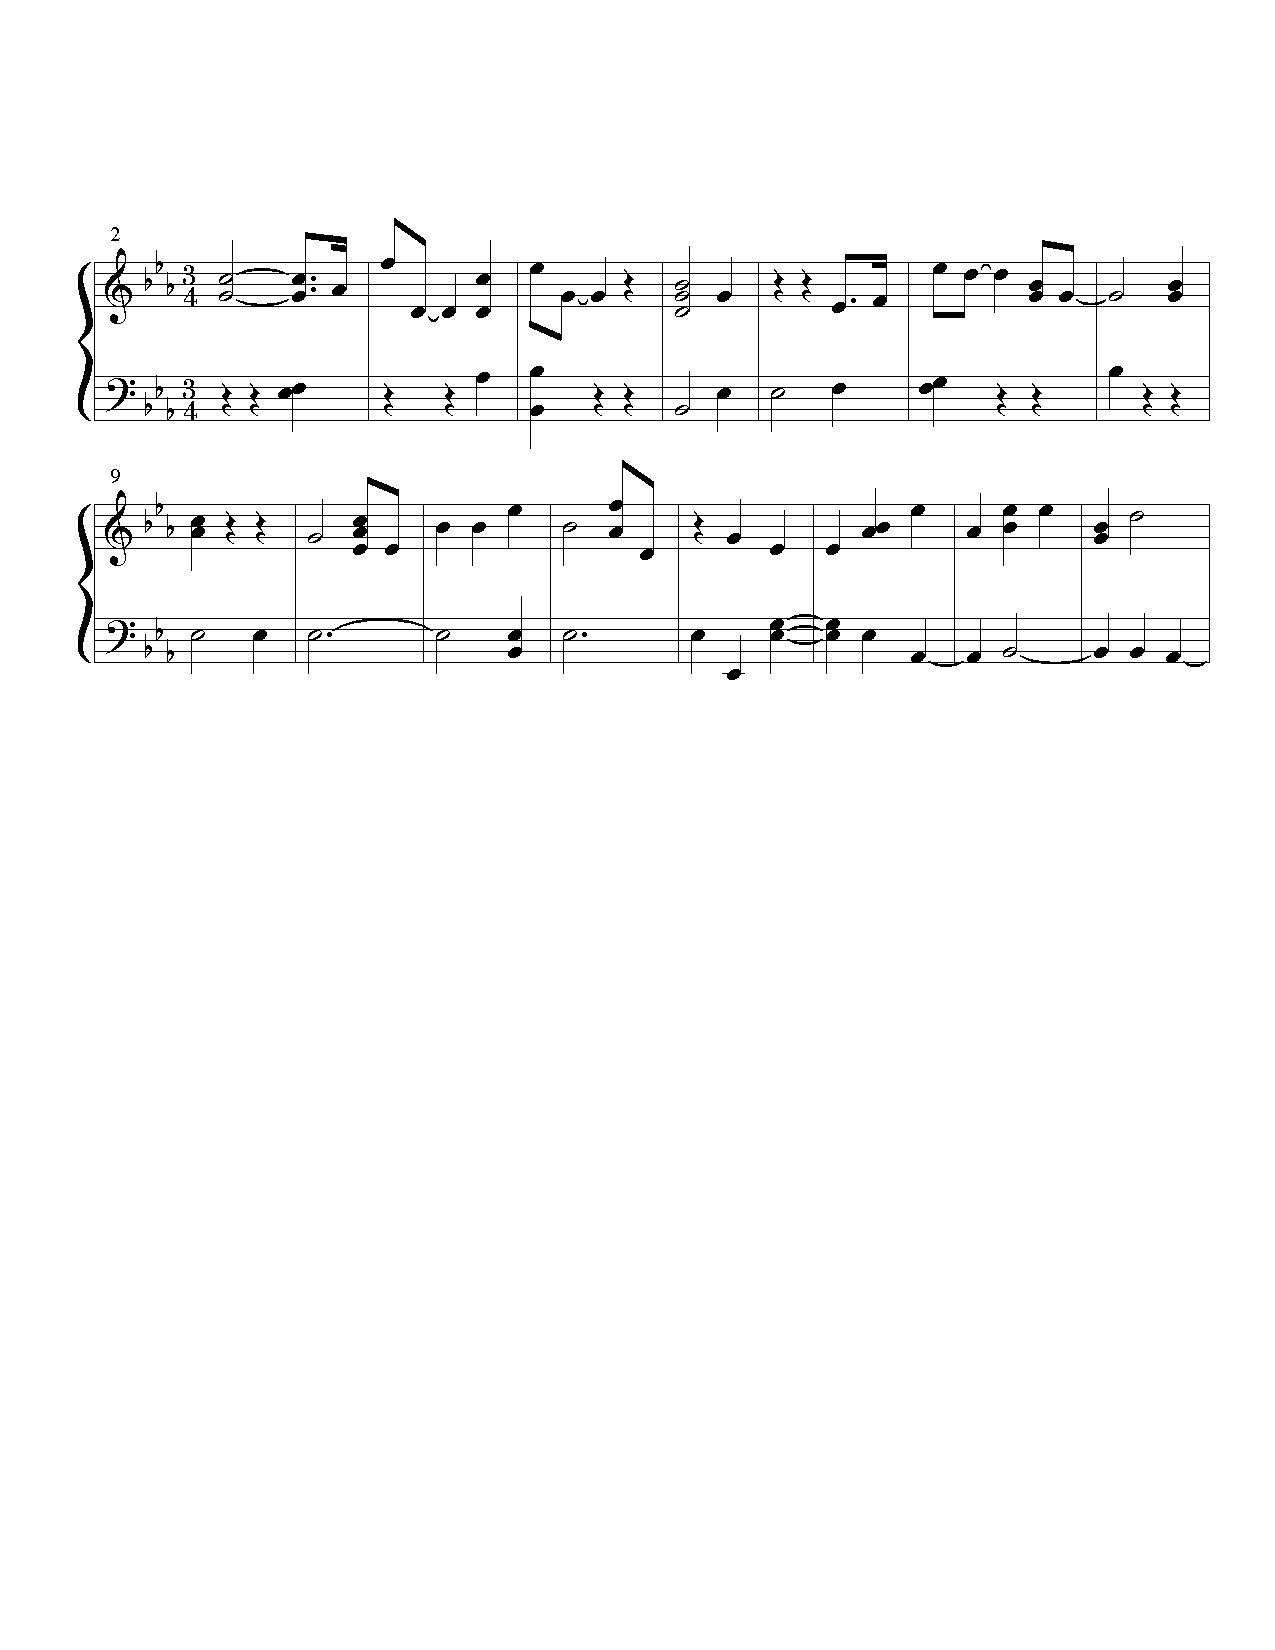
\includegraphics [scale = 0.6] {JupiterRemix2-cropped.pdf}
\caption{Jupiter Remix - Model 2\label{J2}}
\end{figure}

The Canon composition created using the second order Hidden Markov Model had more sixteenth notes than the first remix, but fewer sixteenth notes than the original version ({\autoref{P2}}). There were still awkward interval jumps present in the piece. Overall, the chords made more sense and there was less dissonance in this piece than the first remix. The progression of the generated song seemed to be more logical than the first model. This probably occurred because the second order HMM captured more structure than the first order HMM.

\subsection{Model 3: First Order Hidden Markov Model with Two Hidden States}

Of the three remixes, this version had the fewest rests of the remixed compositions, but more than the original version (\autoref{J3}). It also contained large interval jumps. These jumps between notes were larger than those that occurred in the original song, but tended to be smaller than the jumps in the other versions. 


\begin{figure}[H]
\centering

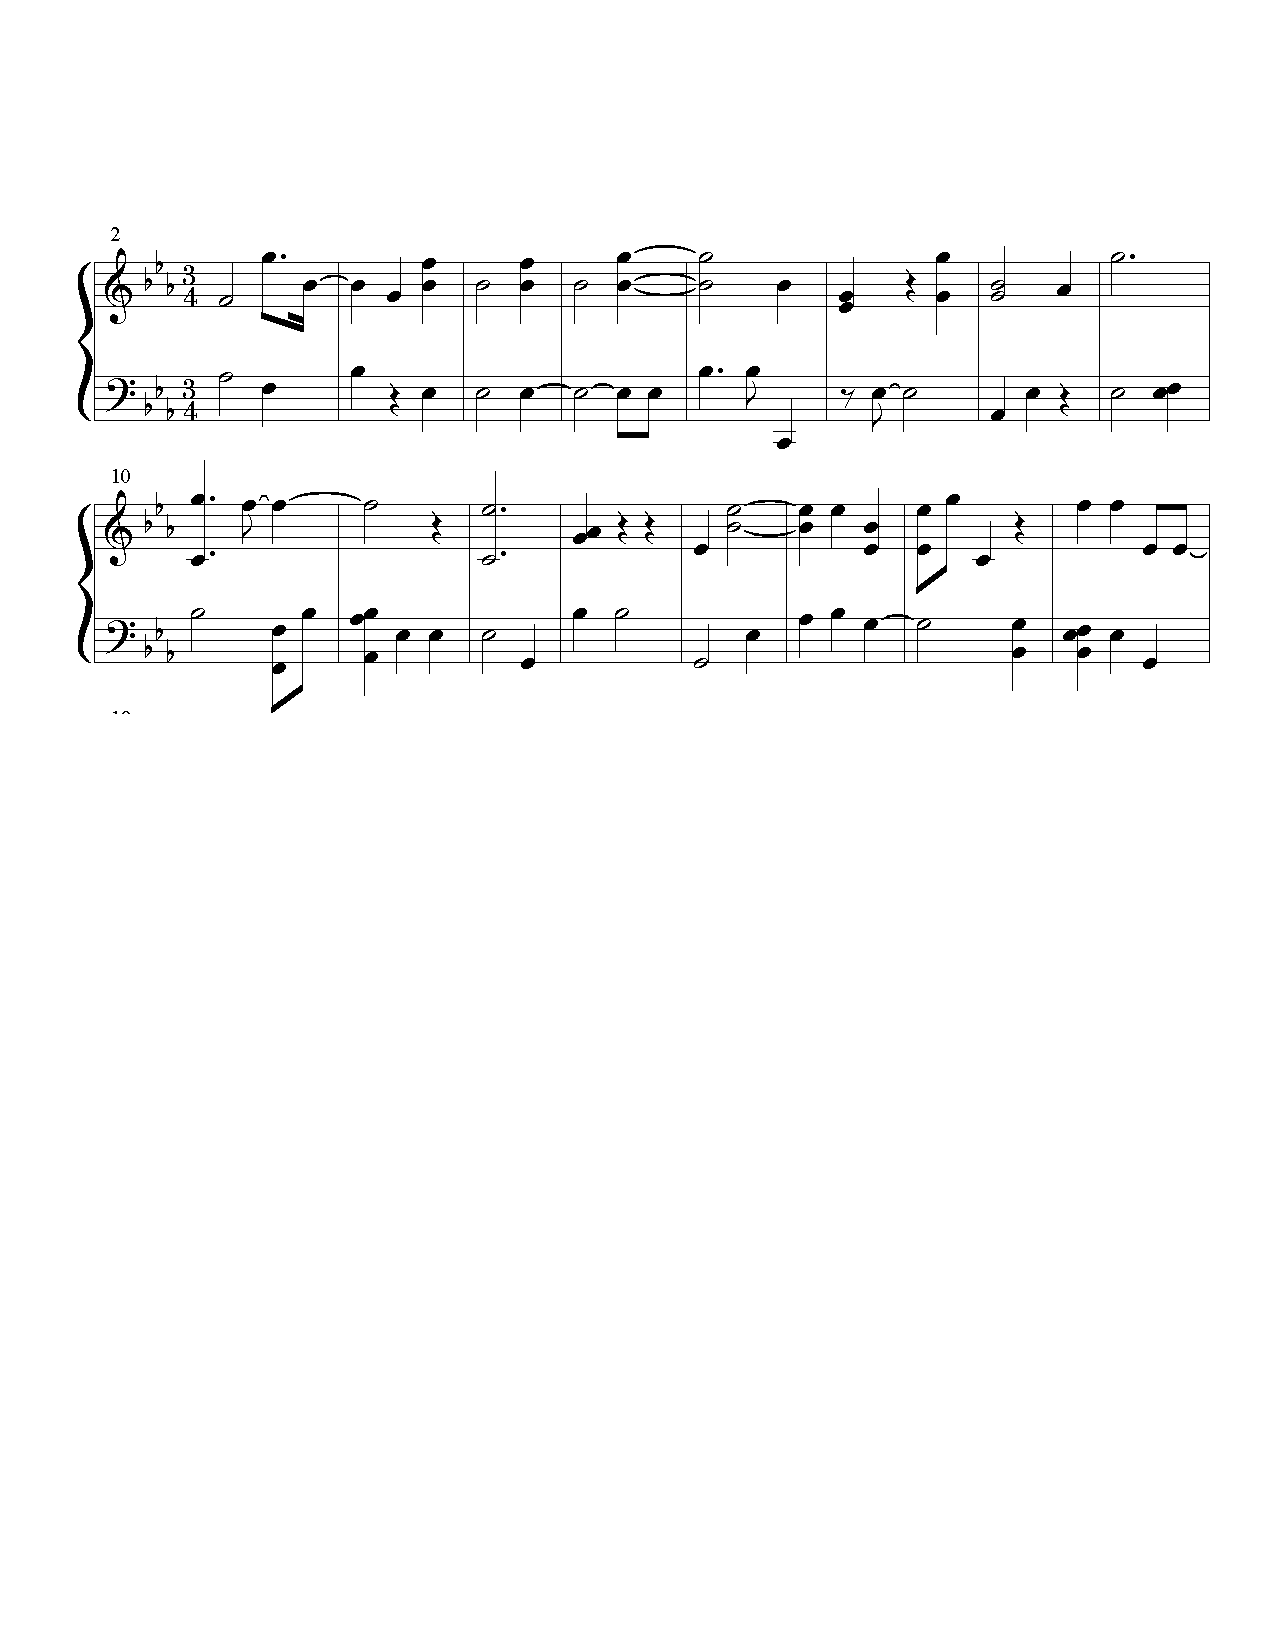
\includegraphics [scale = 0.6] {JupiterRemix2H-cropped.pdf}
\caption{Jupiter Remix - Model 3\label{J3}}
\end{figure}

Likewise, for Pachelbel's Canon, the two latent state version had more eighth and sixteenth notes than the other two remix versions (\autoref{P3}). However, it still did not have as many as the original version and there were still large interval jumps  between successive notes. 

The following figures (\autoref{JV0}, \autoref{JV1}, \autoref{JV2}, \autoref{JV3}) display the velocities for successive notes of the original compositions and the remixes. The same figure can be found in the Appendix for  Pachelbel's Canon (\autoref{PV0}). 


For the original Jupiter piece, the velocity appears to be approximately randomly scattered about 80 with a few outliers but no apparent structure.  For Model 1 and Model 2, however, there appeared to be significant structure in the velocity over time. There were straight lines of constant velocity that were not present in the original piece.  Finally, Model 3 (2 hidden states) appeared to best replicate the velocity found in the original piece, as the velocities again appeared randomly scattered, though perhaps with slightly more structure than originally.

For Pachelbel's Canon, the velocities increased to about the middle of the original piece and then decreased again in a parabola-like shape.  None of the three models were able to recreate this pattern in the velocity and they all had significant, straight structure and much less variation in velocity than the original piece.


\begin{figure}[ht] 
  \label{ fig7} 
  \begin{minipage}[b]{0.5\linewidth}
    \centering
    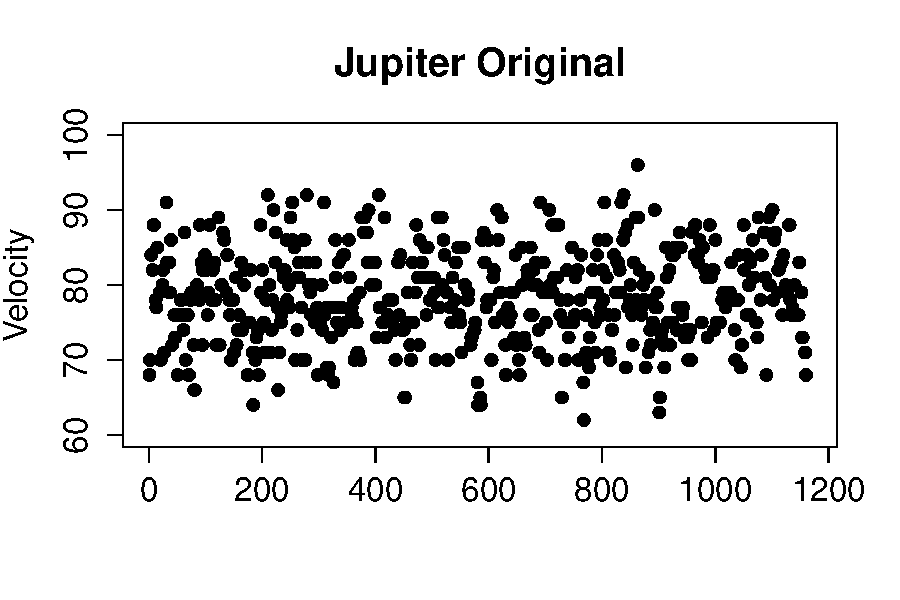
\includegraphics[scale = 0.45]{JupiterOriginalVelocity.pdf} 
    \caption{Initial condition\label{JV0}} 
    \vspace{4ex}
  \end{minipage}%%
  \begin{minipage}[b]{0.5\linewidth}
    \centering
    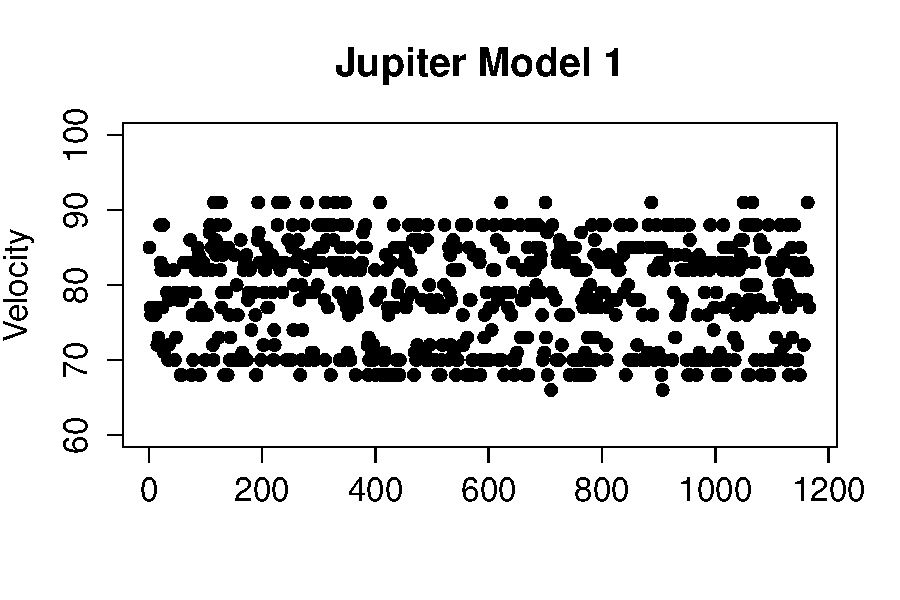
\includegraphics[scale = 0.45]{JupiterModel1Velocity.pdf} 
    \caption{First Order HMM\label{JV1}} 
    \vspace{4ex}
  \end{minipage} 
  \begin{minipage}[b]{0.5\linewidth}
    \centering
    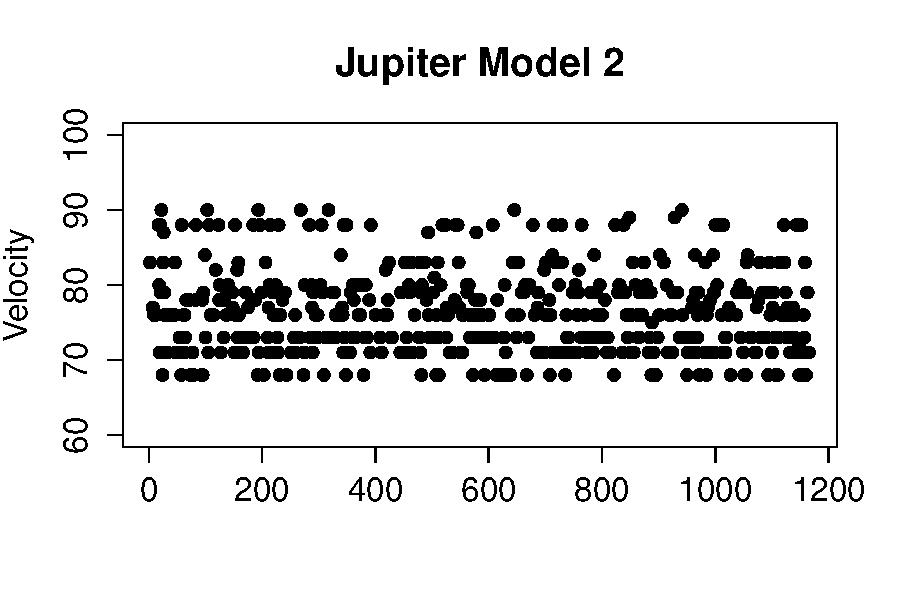
\includegraphics[scale = 0.45]{JupiterModel2Velocity.pdf} 
    \caption{Second Order HMM\label{JV2}} 
    \vspace{4ex}
  \end{minipage}%% 
  \begin{minipage}[b]{0.5\linewidth}
    \centering
    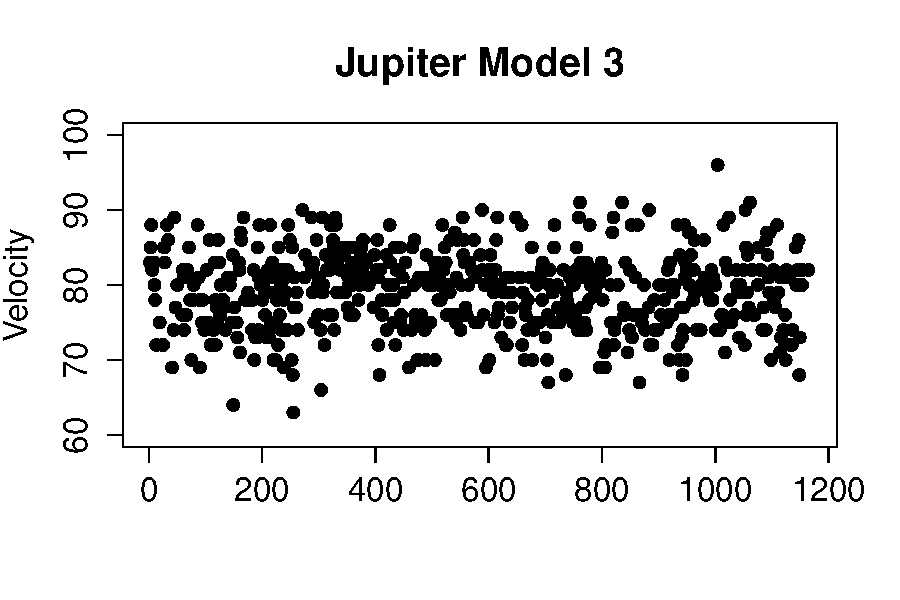
\includegraphics[scale = 0.45]{JupiterModel3Velocity.pdf} 
    \caption{Two Hidden States\label{JV3}} 
    \vspace{4ex}
  \end{minipage} 
\end{figure}

\subsection{Summary}

Overall, the remix generated using the second order Hidden Markov Model appeared to have the best musical structure of all of the remixes, while the remix created using the first order Hidden Markov Model with two latent states had better musical chords. In all of the new compositions, the melody seemed to be split between the two hands. The models did not catch the general structure that lower notes, those played by the left hand, were longer in the original versions of the pieces and tended to be accompaniment, while most of the melody was in the notes played by the right hand. In all of the models, the dynamics were modeled independently from the pitches and as a result the dynamics did not always occur in a logical fashion. There were many instances where certain notes were uncomfortably loud compared to the rest of the piece and did not logically fit in with the rest of the generated piece. 

Twenty-two individuals were sent the three versions of one of the two original songs and were asked which version they preferred (\autoref{survey1}) as well as which original song, Jupiter or Pachelbel's Canon, they thought generated the new versions (\autoref{survey2}). Of the listeners asked about the compositions inspired by Pachabel's Canon, three preferred Model 1, six preferred Model 2 and only one preferred Model 3. Six out of ten correctly identified the original composition.  Of those that listened to Jupiter, none of the respondents preferred Model 1, ten preferred Model 2 and two preferred Model 3. Eight of twelve respondents correctly chose Jupiter as the original composition for the other remixes. 
For both groups, Model 2, the second order HMM,  was by far the overall preferred composition.  

Full MP3 versions of all generated songs, as well as the original versions of Jupiter and Pachelbel's Canon are included with the paper.  As above, in the naming of the MP3s, Model 1 refers to the first order HMM, Model 2 to the second order HMM and Model 3 to the two hidden state HMM.




\begin{figure}
\centering
\begin{subfigure}{.5\textwidth}
  \centering
  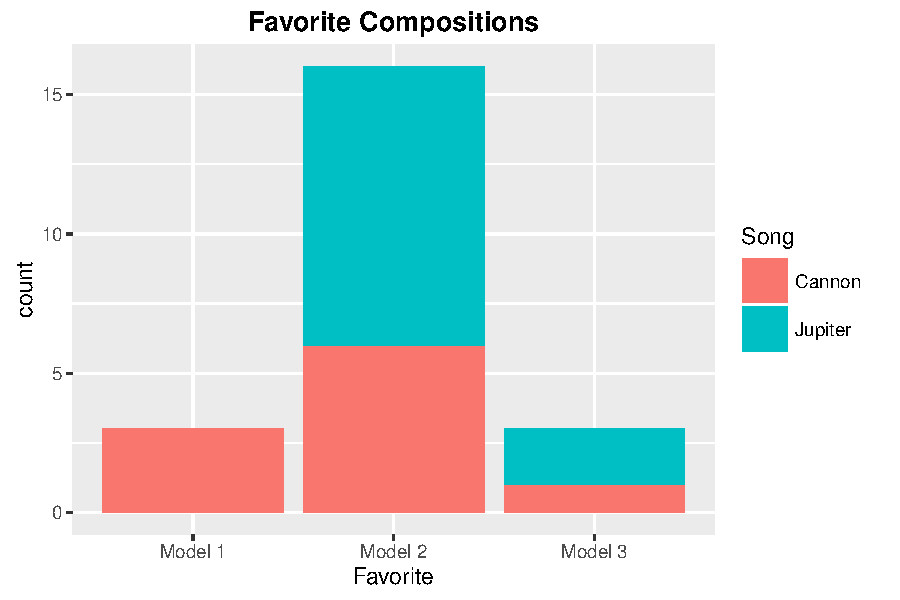
\includegraphics[scale = 0.5]{SurveyFav.pdf}
  \caption{Preferred Compositions\label{survey1}}
  \label{fig:sub1}
\end{subfigure}%
\begin{subfigure}{.5\textwidth}
  \centering
  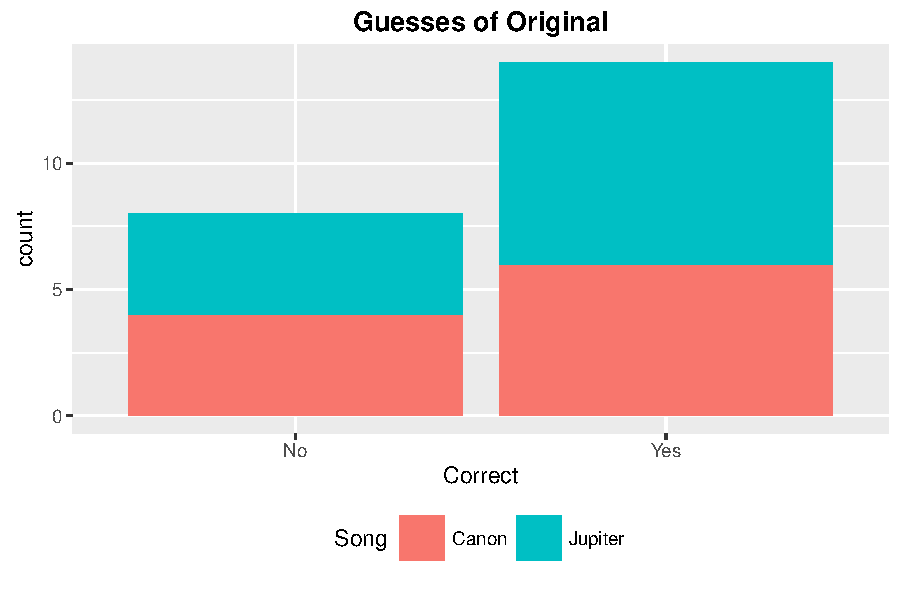
\includegraphics[scale = 0.5]{SurveyGuesses.pdf}
  \caption{Inspiration for the Remixes\label{survey2}}
  \label{fig:sub2}
\end{subfigure}
\caption{Survey Results}
\label{fig:test}
\end{figure}




\section{Conclusion and Further Research}

Of the three models used to create the remixed compositions, none of the models produced pieces that sounded like coherent music throughout the duration of the generated piece. There was not a remix that told a story or evoked an emotion, like the originals. This was not surprising given the relatively simple structures of our models. There were certain points in some of the pieces where individual measures sounded good, but the overall piece still was not as cohesive as we would have liked. The second order HMM seemed to perform the best in creating music. 

One extension of this project we would like to explore is the application of higher order Hidden Markov Models. Models of higher orders would allow for the current note pitches and velocities to depend on more previous states and capture more complex musical theory. This would introduce more structure and dependence into the models that could create the cohesion in the pieces that was missing above. The second order HMM seemed to perform the best, so it would be interesting to see how a third, fourth or fifth order HMM could improve the generated compositions. 

In addition, we need to include the dependencies between the dynamics and the notes in the model. This could improve the disconcerting loud notes in the pieces. Modeling such dependency could also extend to orchestral pieces with multiple instruments. This would require the dependencies between instruments to be modeled as well. Increasing the number of hidden states for our current model might also improve our results, but this requires more computational power or optimization of the current code.

The resulting compositions from these models showed promising results, but there is significant room for improvement. The improvements and extensions described above could elevate our results to more cohesive and complicated compositions that have more of a resemblance to actual music composition. 


\newpage

\section{Appendix}

\subsection{Baum-Welch Algorithm for Second Order HMM}
\label{2ndHMM}
1. Run first order Baum-Welch to estimate $\pi$, T, $\phi$. \newline
2. Use second order Baum-Welch to estimate $T_{ijk}$:\newline

Forward Algorithm: \newline
$$\alpha_1(i) = \pi_i \phi_i(X_1)$$
$$\alpha_2(i,j) = \alpha_1(i) T_{ij} \phi_j(X_2)$$
$$:$$
$$:$$
$$\alpha_{t+1}(j, l) = \sum_{i=1}^m \alpha_t(i,j) T_{ijl} \phi_l(X_{t+1})$$
where 2 $\leq$ t $\leq$ T-1 and 1 $\leq$j,k $\leq$  m. \newline
Thus, $\mathbb{P}(X | \lambda) = \sum_{i=1}^m \alpha_T(i,m)$. \newline

Backward Algorithm: \newline
$$\beta_t(i,j) = \sum_{i=1}^m \beta_{t+1}(j,k) T_{ijk} \phi_k(X_{t+1})$$
where 2 $\leq$ t $\leq$ T-1 and 1 $\leq$ j,k $\leq$ m. \newline

Baum-Welch Estimate for $T_{ijk}$: \newline
$$\bar{T}_{ijk} = \frac{\sum_t \beta_t (i,j,k)}{\sum_{k,t} \beta_t (i,j,k)}$$
where 2 $\leq$ t $\leq$ T-1 and \newline
$$\beta_t(i,j,k) = \frac{\alpha_t(i,j) T_{ijk} \phi_k(x_{t+1}) \beta_{t+1}(j,k)}{\mathbb{P}(x|\lambda)}$$ 




Iterate until convergence. 

\subsection{Baum-Welch for First Order HMM with Two Hidden States}
\label{3rdHMM}
Define the following:

$$A_{ij} = \mathbb{P} (R_t = j | R_{t-1} = i)$$
$$B_{jkl} = \mathbb{P} (S_t = l | R_t = j, S_{t-1} = k)$$ 
$$T_{ik, jl} = A_{ij} B_{jkl} = \mathbb{P} (R_j = j, S_t = l | R_{t-1} = i, S_{t-1} = k)$$
$$Z_t = (R_t, S_t)$$

The constraints are $\sum_j A_{ij} = 1, \sum_l B_{jkl} = 1.$ \newline

Define c to be a constant. Then,  \newline
$$Q(\theta, \theta_k) = c + \sum_{t=2}^n \sum_{i,k} \sum_{j,l} \mathbb{P}_{\theta_k} (R_{t-1} = i, S_{t-1} = k, R_t = j, S_t = l | X) \log T_{ik, jl}$$ 
Let $$B_{t,ik,jl} = \mathbb{P}_{\theta_k} (R_{t-1} = i, S_{t-1} = k, R_t = j, S_t = l | X).$$ We have that $$\log T_{ik, jl} = \log A_{ij} + \log B_{jkl}.$$

Thus, \newline
$$ 0 = \frac{\partial}{\partial A_ij}(Q(\theta, \theta_k) - \lambda \sum_{j} A_{ij}) = (\sum_{t=2}^n \sum_k \sum_l B_{t,ik,jl} \frac{1}{A_{ij}}) - \lambda$$
$$\lambda A_{ij} = \sum_{t=2}^n \sum_k \sum_l B_{t,ik,jl}$$
$$\lambda = \sum_j \sum_{t=2}^n \sum_k \sum_l B_{t,ik,jl}$$

For each i, $$A_{ij} \propto \sum_{t=2}^n \sum_{k,l} B_{t,ik,jl}$$ \newline

$$ 0 = \frac{\partial}{\partial B_{jkl}} (Q(\theta, \theta_k) - \lambda \sum_l B_{jkl}) = \sum_{t=2}^n \sum_i B_{t,ik,jl} \frac{1}{B_{jkl}} - \lambda$$
$$ \lambda B_{jkl} = \sum_{t=2}^n \sum_i B_{t,ik,jl}$$

For each j, k, \newline
$$B_{jkl} \propto \sum_{t=2}^n \sum_i B_{t,ik,jl}$$

\subsection{Pachabel's Canon Resuts}

\begin{figure}[H]
\centering

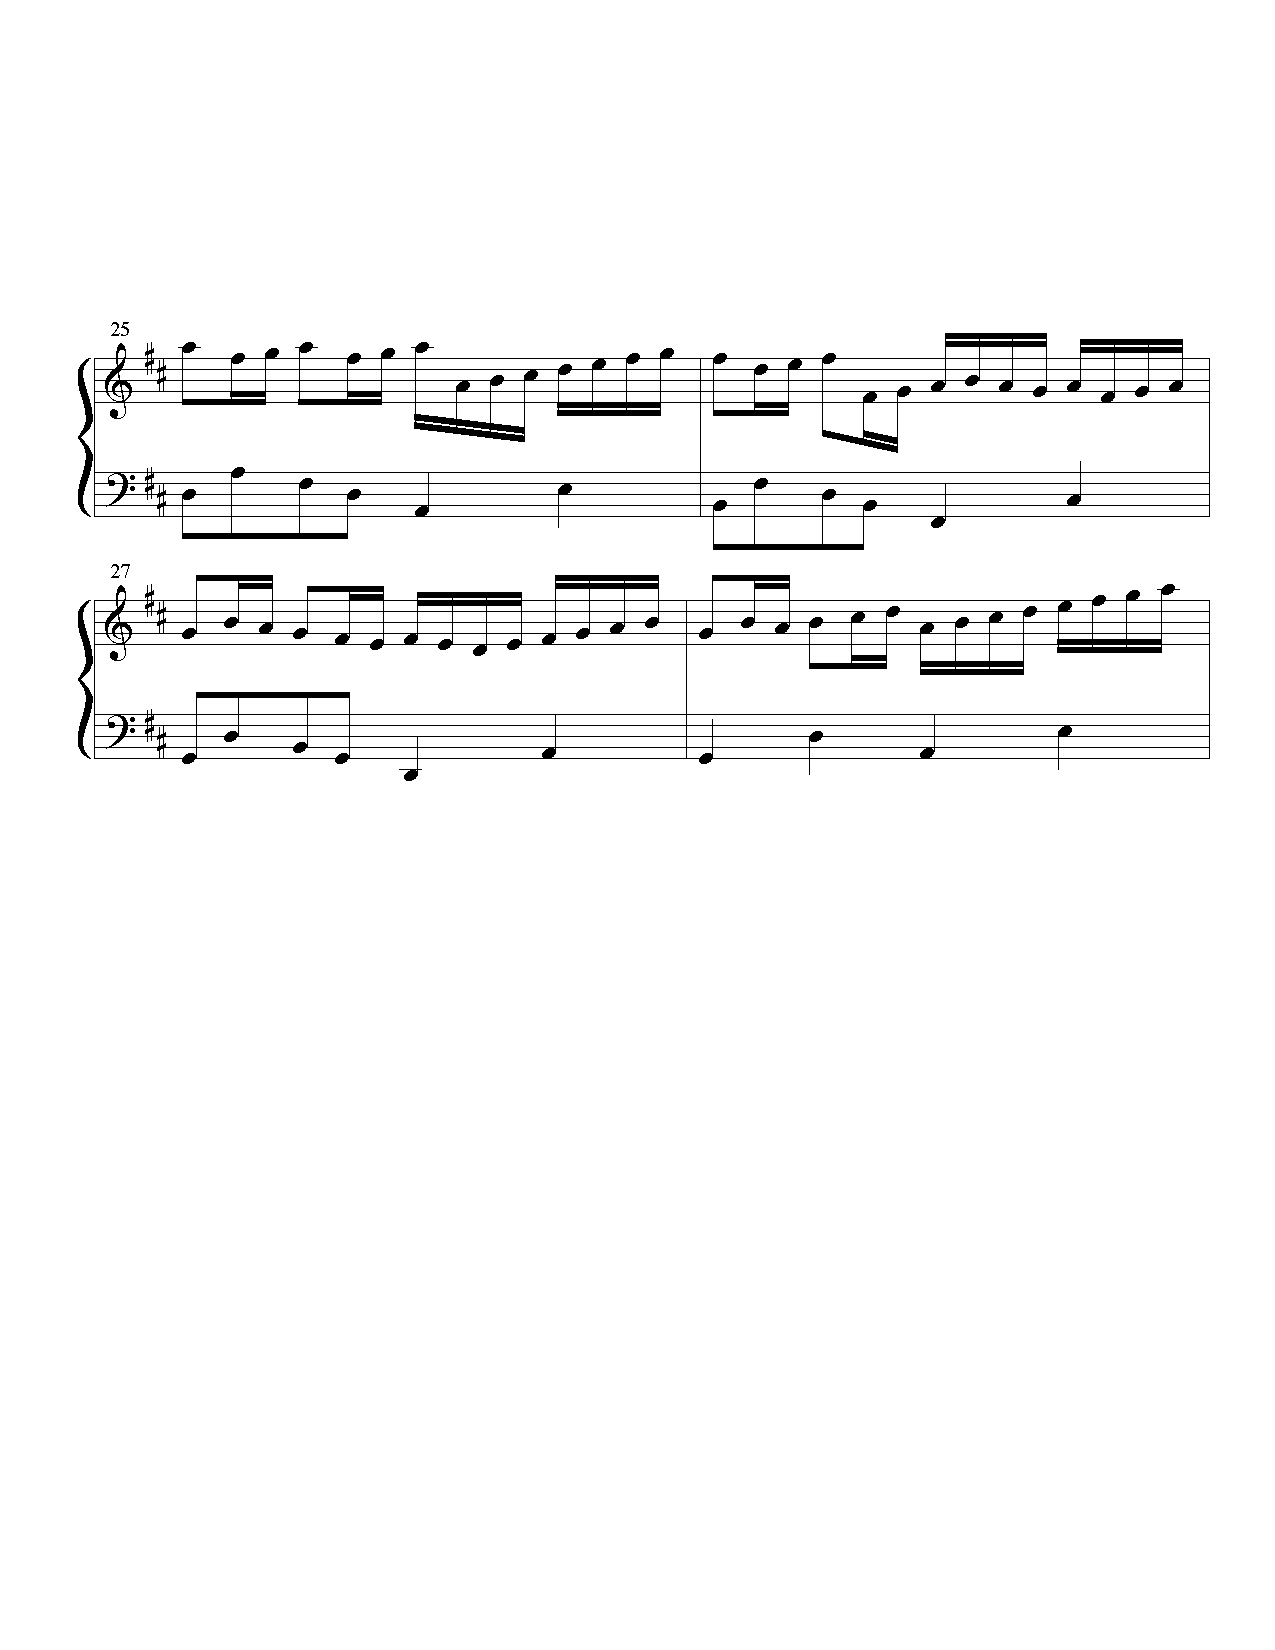
\includegraphics [scale = 0.6] {PachelbelOriginal-cropped.pdf}
\caption{Pachelbel Original\label{Porig}}
\end{figure}

\begin{figure}[H]
\centering

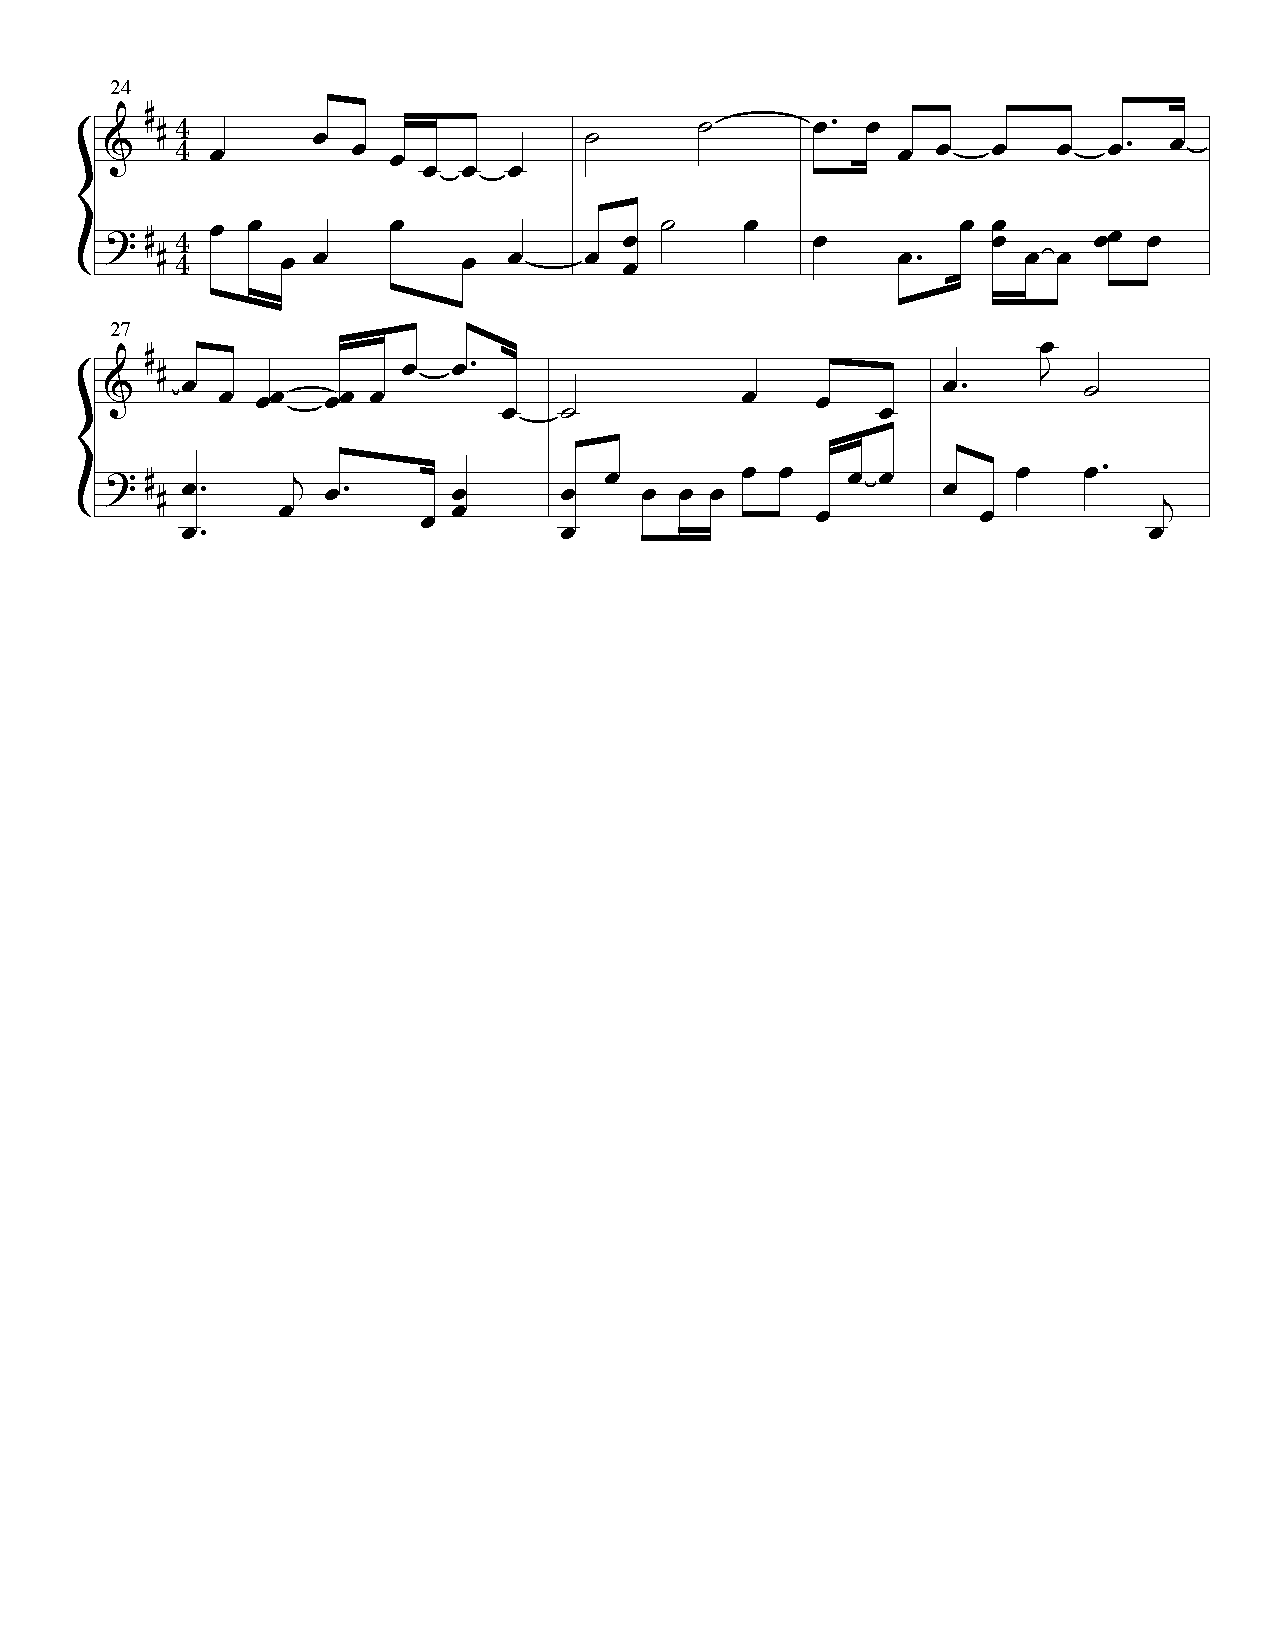
\includegraphics [scale = 0.6] {PachelbelRemix-cropped.pdf}
\caption{Pachelbel Remix - Model 1\label{P1}}
\end{figure}

\begin{figure}[H]
\centering

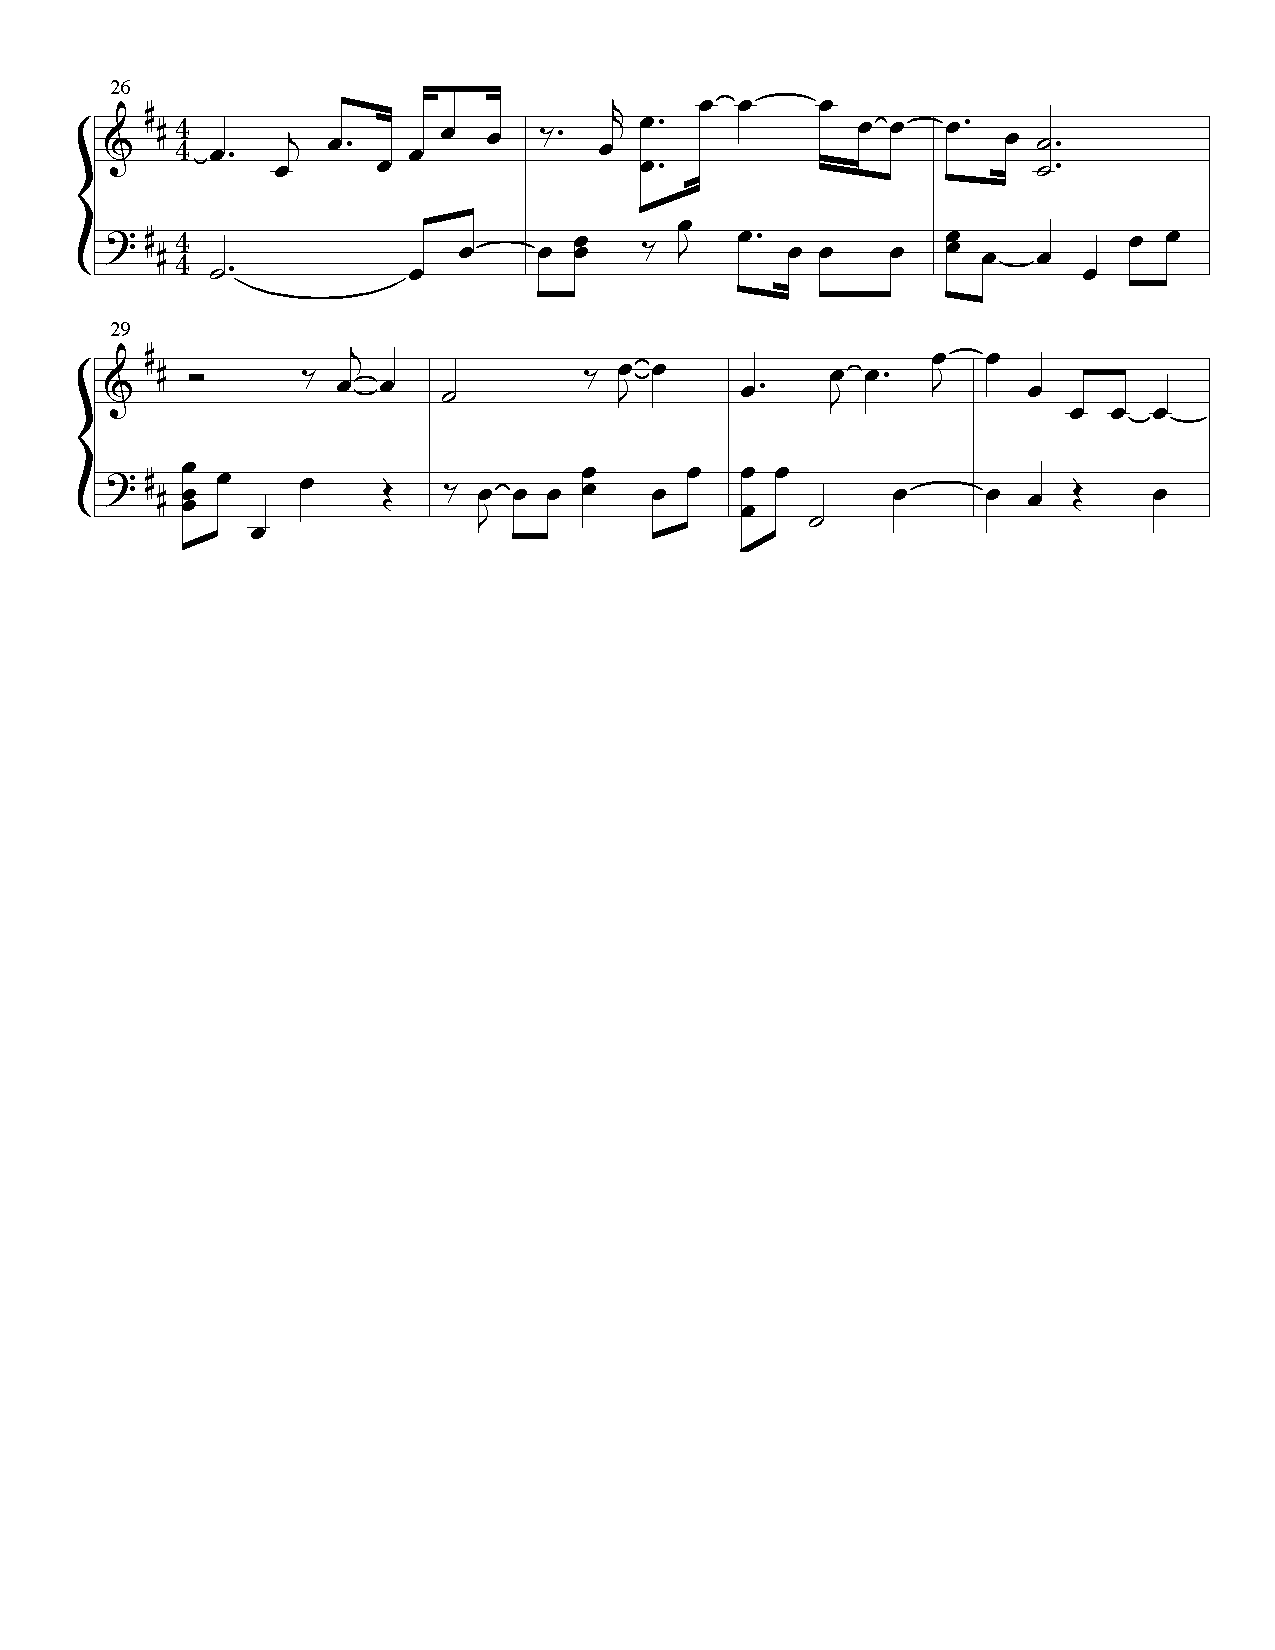
\includegraphics [scale = 0.6] {PachelbelRemix2-cropped.pdf}
\caption{Pachelbel Remix - Model 2\label{P2}}
\end{figure}

\begin{figure}[H]
\centering

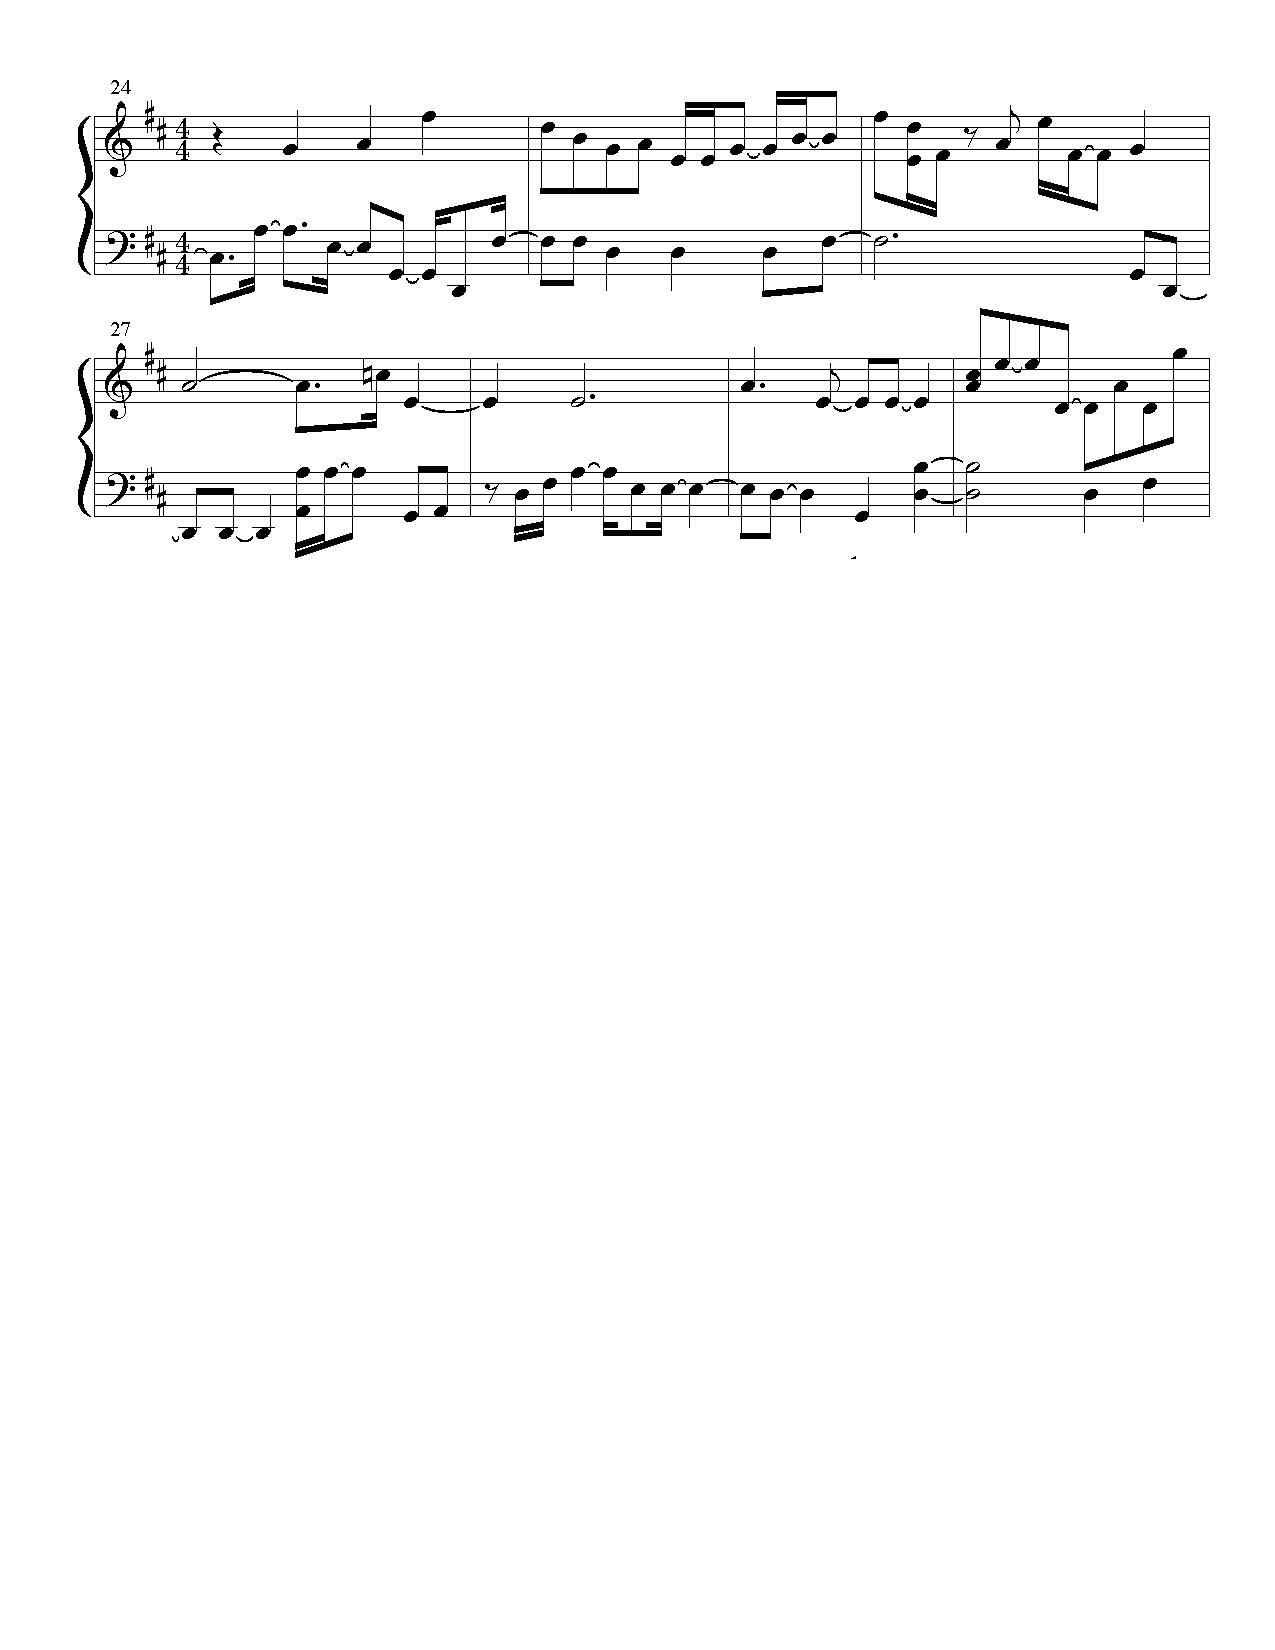
\includegraphics [scale = 0.6] {PachelbelRemix2H-cropped.pdf}
\caption{Pachelbel Remix - Model 3\label{P3}}
\end{figure}


\begin{figure}[ht] 
  \label{ fig7} 
  \begin{minipage}[b]{0.5\linewidth}
    \centering
    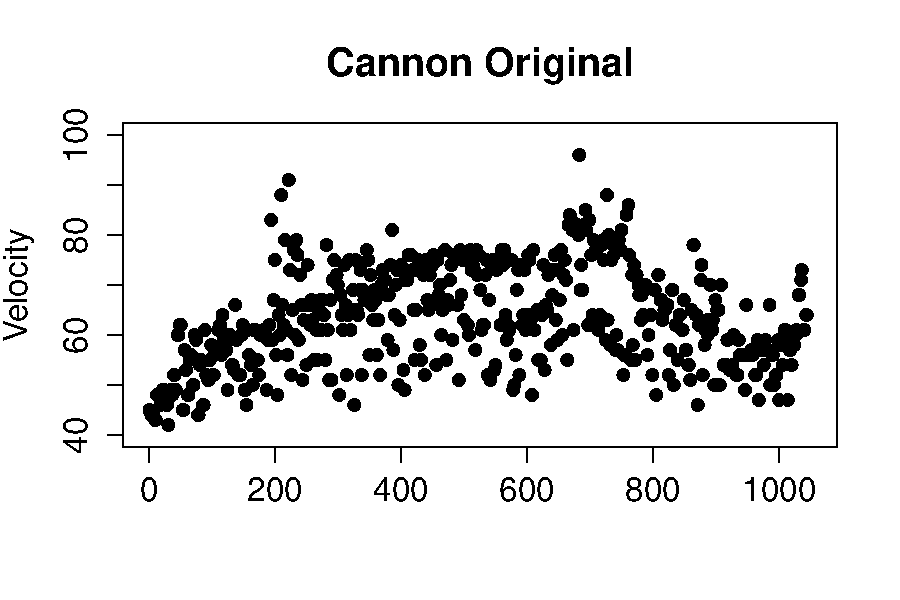
\includegraphics[scale = 0.45]{CannonOriginalVelocity.pdf} 
    \caption{Initial condition\label{PV0}} 
    \vspace{4ex}
  \end{minipage}%%
  \begin{minipage}[b]{0.5\linewidth}
    \centering
    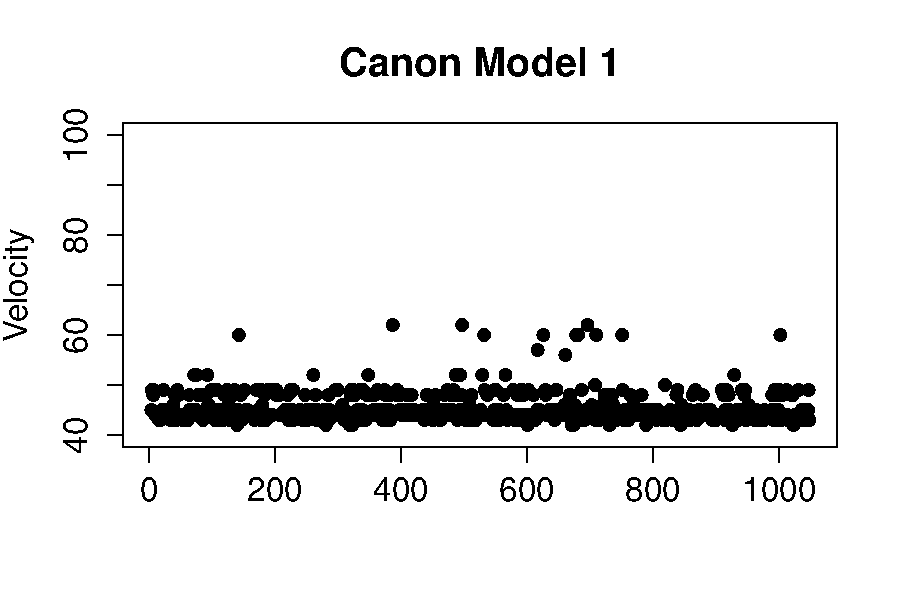
\includegraphics[scale = 0.45]{CannonModel1Velocity.pdf} 
    \caption{First Order HMM\label{PV1} }
    \vspace{4ex}
  \end{minipage} 
  \begin{minipage}[b]{0.5\linewidth}
    \centering
    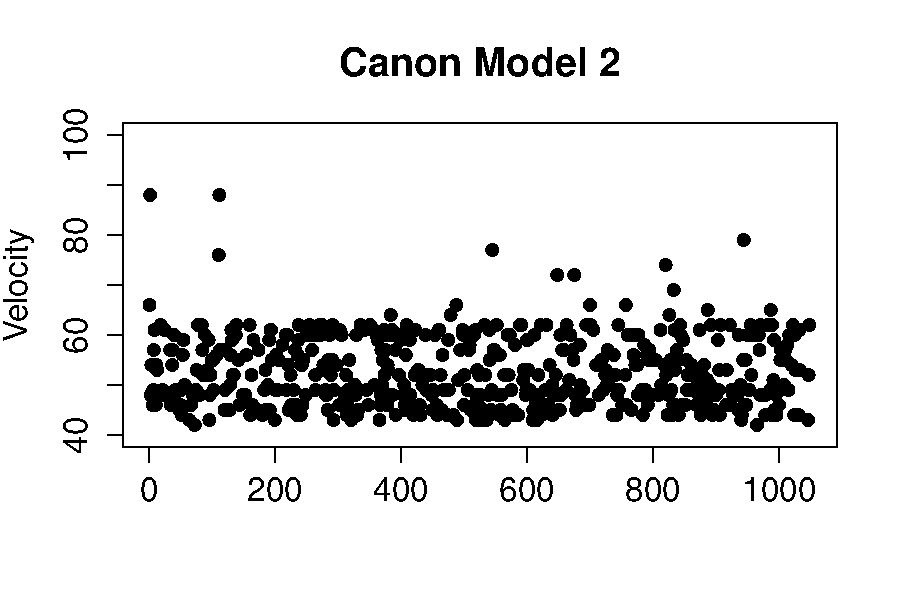
\includegraphics[scale = 0.45]{CannonModel2Velocity.pdf} 
    \caption{Second Order HMM} 
    \vspace{4ex}
  \end{minipage}%% 
  \begin{minipage}[b]{0.5\linewidth}
    \centering
    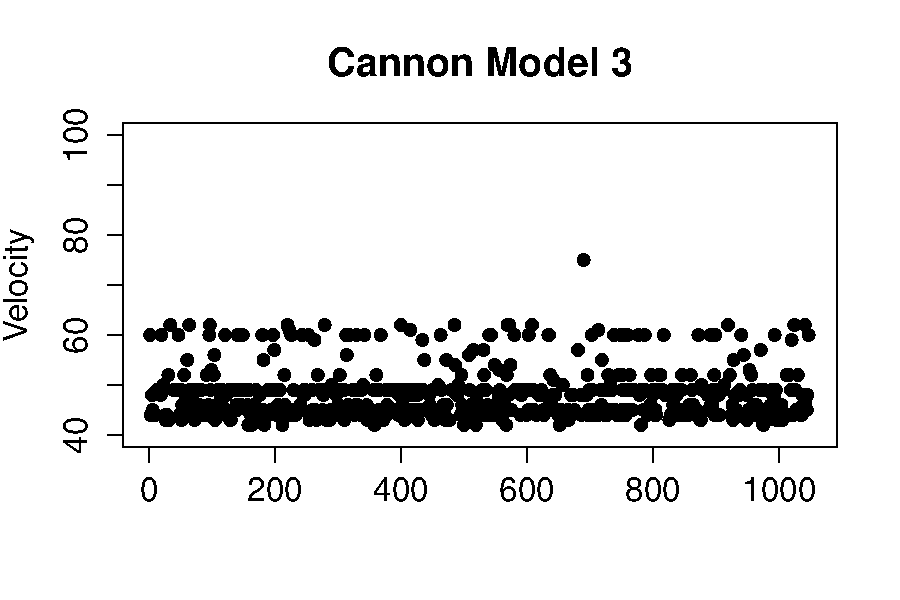
\includegraphics[scale = 0.45]{CannonModel3Velocity.pdf} 
    \caption{Two Hidden States} 
    \vspace{4ex}
  \end{minipage} 
\end{figure}

\newpage

\section{References}
\begin{enumerate}

\item MIDI Manufacturers Association, "An Introduction to Midi". 
\item Music Composition for Dummies, http://www.dummies.com/how-to/content/music-composition-for-dummies-cheat-sheet.html
\item MIDI to CSV: \url{http://www.fourmilab.ch/webtools/midicsv/}
\item Hidden Markov Models, Statistics 531, Duke University Spring 2016. Instructor: Jeff Miller
\item Jean-Francoix Mari and Rene Schott, "Probabilistic and Statistical Methods in Computer Science", Springer Science, pg. 161-167.  
\item Brett Watson and Ah Chung Tsoi, "Second Order Hidden Markov Models for Speech Recognition", University of Queensland, 146 - 151.
\end{enumerate}

\end{document}